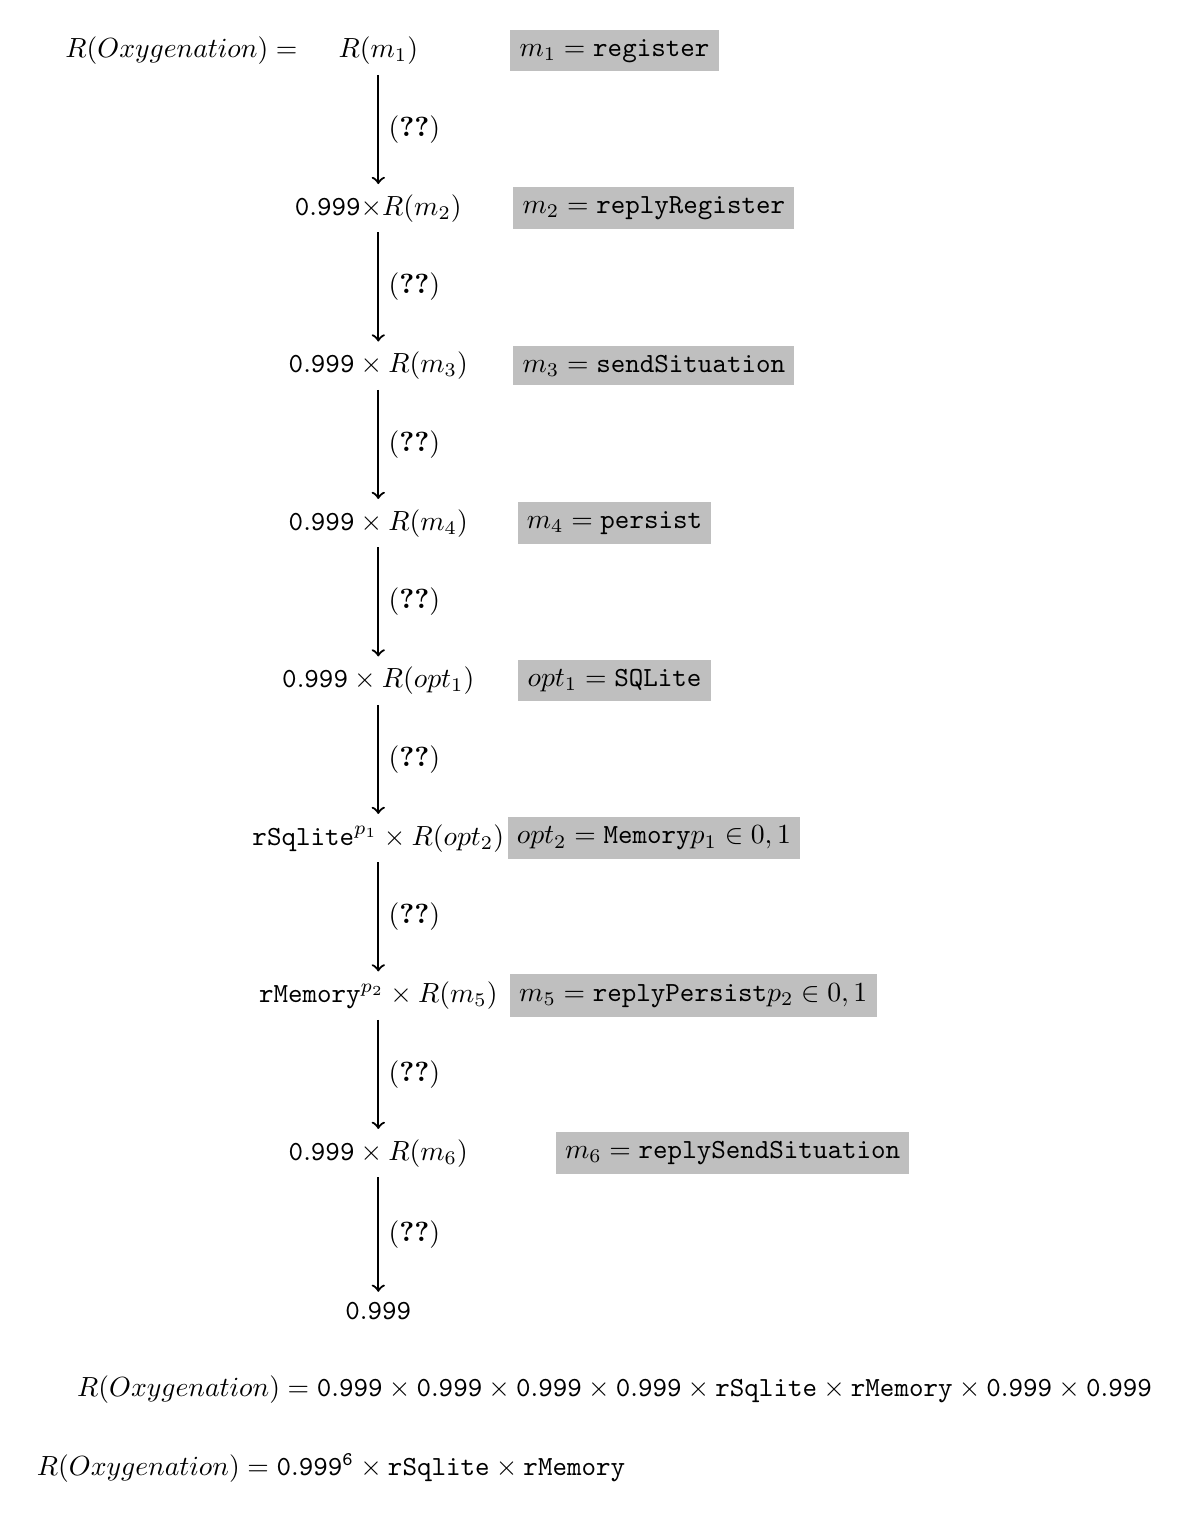
\begin{tikzpicture}[thick]
%\draw[help lines, step=1cm] (0,0) grid +(10,15);
%%%%%%%%%%%%%%%%%%%%%%%%%%%%%%% Derivation tree for SQLite
\node[rectangle, draw=none](rOxygenation) at (-0.5,15){$R(Oxygenation)=$};
\node[rectangle, draw=none](rM1) at (2,15){$R(m_1)$};
\node[rectangle, draw=none, fill=gray!50](obsM1) at(5,15){$m_1 = \mathtt{register}$};
\node[rectangle, draw=none](rM2) at(2,13){$\mathtt{0.999 \times} R(m_2)$};
\node[rectangle, draw=none, fill=gray!50](obsM1) at(5.5,13){$m_2 = \mathtt{replyRegister}$};
\draw[->, thick] (rM1) -- node[draw=none, auto]{(\ref{eq:syncMessageReliability})}(rM2);
\node[rectangle, draw=none](rM3) at(2,11){$\mathtt{0.999} \times R(m_3)$};
\node[rectangle, draw=none, fill=gray!50](obsM1) at(5.5,11){$m_3 = \mathtt{sendSituation}$};
\draw[->, thick] (rM2) -- node[draw=none, auto]{(\ref{eq:syncMessageReliability})}(rM3);

\node[rectangle, draw=none](rM4) at(2,9){$\mathtt{0.999} \times R(m_4)$};
\node[rectangle, draw=none, fill=gray!50](obsM4) at(5,9){$m_4 = \mathtt{persist}$};
\draw[->, thick] (rM3) -- node[draw=none, auto]{(\ref{eq:syncMessageReliability})}(rM4);
\node[rectangle, draw=none](rOpt1) at(2,7){$\mathtt{0.999} \times R(opt_1)$};
\node[rectangle, draw=none, fill=gray!50](obsOpt1) at(5,7){$opt_1 = \mathtt{SQLite}$};
\draw[->, thick] (rM4) -- node[draw=none, auto]{(\ref{eq:syncMessageReliability})}(rOpt1);
\node[rectangle, draw=none](rOpt2) at(2,5){$\mathtt{rSqlite}^{p_1} \times R(opt_2)$};
\node[rectangle, draw=none, fill=gray!50](obsOpt2) at(5.5,5){$opt_2 = \mathtt{Memory}$\\$p_1 \in {0,1}$};
\draw[->, thick] (rOpt1) -- node[draw=none, auto]{(\ref{eq:optionalFragmentReliability})}(rOpt2);
\node[rectangle, draw=none](rM5) at(2,3){$\mathtt{rMemory}^{p_2} \times R(m_5)$};
\node[rectangle, draw=none, fill=gray!50](obsOpt2) at(6,3){$m_5 = \mathtt{replyPersist}$\\$p_2 \in {0,1}$};
\draw[->, thick] (rOpt2) -- node[draw=none, auto]{(\ref{eq:optionalFragmentReliability})}(rM5);
\node[rectangle, draw=none](rM6) at(2,1){$\mathtt{0.999} \times R(m_6)$};
\node[rectangle, draw=none, fill=gray!50](obsM6) at(6.5,1){$m_6 = \mathtt{replySendSituation}$};
\draw[->, thick] (rM5) -- node[draw=none, auto]{(\ref{eq:syncMessageReliability})}(rM6);
\node[rectangle, draw=none](rTerm) at(2,-1){$\mathtt{0.999}$};
% \node[rectangle, draw=none, fill=gray!50](obsTerm) at(5.5,1){$m_6 = \mathtt{replySendSituation}$};
\draw[->, thick] (rM6) -- node[draw=none, auto]{(\ref{eq:syncMessageReliability})}(rTerm);

\node[rectangle, draw=none](rOxygenation) at (5,-2){$R(Oxygenation)= \mathtt{0.999 \times 0.999 \times 0.999 \times 0.999 \times rSqlite \times rMemory \times 0.999 \times 0.999}$};
\node[rectangle, draw=none](rOxygenation) at (1.4,-3){$R(Oxygenation)= \mathtt{0.999^6 \times rSqlite \times rMemory }$};
\end{tikzpicture}
